\documentclass[UTF8]{ctexart}
\ctexset { section = { format={\Large \bfseries } } }
\pagestyle{plain}
\usepackage{float}
\usepackage{amsmath}
\usepackage{amssymb}
\usepackage{listings}
\usepackage{graphicx}
\usepackage{xcolor}
\usepackage{geometry}
\geometry{a4paper,scale=0.8}
\usepackage{caption}
\captionsetup[figure]{name={Figure}}

\lstset{
language=Python, % 设置语言
basicstyle=\ttfamily, % 设置字体族
breaklines=true, % 自动换行
keywordstyle=\bfseries\color{blue}, % 设置关键字为粗体,
morekeywords={}, % 设置更多的关键字,用逗号分隔
emph={self}, % 指定强调词,如果有多个,用逗号隔开
emphstyle=\bfseries\color{Rhodamine}, % 强调词样式设置
commentstyle=\color{black!50!white}, % 设置注释样式,斜体,浅灰色
stringstyle=\bfseries\color{red!90!black}, % 设置字符串样式
columns=flexible,
numbers=left, % 显示行号在左边
numbersep=2em, % 设置行号的具体位置
numberstyle=\footnotesize, % 缩小行号
frame=single, % 边框
framesep=1em % 设置代码与边框的距离
}

\title{\textbf{Data Structure lab3}}
\author{吴嘉骜 21307130203}
\date{\today}

\begin{document}

\maketitle

\noindent
\textbf {Objective}\\  The objective of this lab is to understand the use of stack to evaluate Postfix expression converted from Infix. \\
\noindent
\textbf {Experiment environment} \\
    Windows 11 VsCode Python 3.10.7 64-bit

\section{Coding}
\setlength{\parindent}{0pt}
\subsection{}
Write code for Infix to postfix conversion by using stack (The code should
be able to treat with parenthesis, braces and at least the following operators:
$+, -, \times, /,$ mod).\\
\textbf{Solution}: See infix2post.py.
\begin{lstlisting}
# input: string, infix expression
# output: list, postfix expression
import re

def in2post(infix):
    op_stack = [] # stack to store operators
    result = []  # list to store postfix expression
    ops = ['+', '-', '*', '/', '%', '^', '(', ')', '[', ']', '{', '}']
    op_pri = {
        '+': 1, '-': 1, 
        '*': 2, '/': 2, '%': 2, 
        '^': 3, 
        '(': 0, ')': 0, 
        '[': 0, ']': 0, 
        '{': 0, '}': 0
    }  # updated operator priority
    infix = re.sub(r'(\(|\)|\[|\]|\{|\})', r' \1 ', infix)  # add space around all kinds of brackets
    for token in infix.split(): # split the infix expression by space
        if token not in ops:
            result.append(token)
        elif token in ['(', '[', '{']:
            op_stack.append(token)
        elif token in [')', ']', '}']:
            if token == ')':
                while op_stack[-1] != '(':
                    result.append(op_stack.pop())
            elif token == ']':
                while op_stack[-1] != '[':
                    result.append(op_stack.pop())
            else: # token == '}'
                while op_stack[-1] != '{':
                    result.append(op_stack.pop())
            op_stack.pop()
        else:
            while len(op_stack) != 0 and op_pri[op_stack[-1]] >= op_pri[token]:
                result.append(op_stack.pop())
            op_stack.append(token)
    while len(op_stack) != 0:
        result.append(op_stack.pop())
    return result
\end{lstlisting}
\textbf{Code interpretation:} \\
The code defines a function $in2post$ to convert infix expression to postfix expression. The function takes a string as input and returns a list.
It first defines two lists, $op\_stack$ and $result$, to store operators and postfix expression respectively. Then it defines a dictionary $op\_pri$ to store the priority of operators. 
Next, it adds space around small brackets, square brackets, curly brackets to make it easier to split the infix expression. Then it splits the infix expression by space and iterates the tokens. If the token is not an operator, it appends the token to $result$. 
If the token is a left bracket, it appends the token to $op\_stack$. If the token is a right bracket, it pops operators from $op\_stack$ and appends them to $result$ until it meets the same left bracket. If the token is an operator, it pops operators from $op\_stack$ 
and appends them to $result$ until the priority of the operator in $op\_stack$ is lower than the priority of the token. Finally, it pops all operators from $op\_stack$ and appends them to $result$.\\
As we can see, the code supports three brackets and operators $+, -, \times, /, \% \text{(mod)},\wedge \text{(power)} $.\\


\subsection{}
Write code for Postfix expression evaluation by using stack (Integer division
preserves only the integer part).\\
\textbf{Solution}: See postfixeval.py.
\begin{lstlisting}
# input: string, postfix expression
# output: int, result of the expression
def postfixeval(postfixExpr):
    stack = []
    for token in postfixExpr.split(): # split the postfix expression by space
        if token.isdigit():  # meeting operand, push into stack
            stack.append(int(token))
        # meeting operator, pop two operands and compute
        elif stack:
            try:
                operand2 = stack.pop()
                operand1 = stack.pop()
                result = computing(token, operand1, operand2)
                stack.append(result)
            except:
                print('Error: invalid expression')
                return None
    # finish computing, return the result
    result = stack.pop()
    return result

def computing(operator, oprand1, oprand2):
    if operator == '*':
        return oprand1 * oprand2
    elif operator == '/':
        return oprand1 // oprand2
    elif operator == '+':
        return oprand1 + oprand2
    elif operator == '-':
        return oprand1 - oprand2
    elif operator == '%':
        return oprand1 % oprand2
    elif operator == '^':
        return oprand1 ** oprand2
\end{lstlisting}
\textbf{Code interpretation:} \\
The code defines a function $postfixeval$ to evaluate postfix expression. The function takes a string as input and returns an integer.
It first defines a list $stack$ to store operands. Then it splits the postfix expression by space and iterates the tokens. 
If the token is an operand, it converts the token to an integer and pushes it into $stack$. 
If the token is an operator, it pops two operands from $stack$ and computes the result.
Finally, it returns the result.\\
As we can see, the code supports parenthesis, braces and operators $+, -, \times, /, \% \text{(mod)},\wedge \text{(power)} $.\\



\section{Experiment}
Verify the code through experiments and run these test examples.\\
For code 01, convert the following infix expressions:\\
(a): (A + B) * C\\
(b): A + (B - C)\\
(c): A * (B + C) / D\\
(d): (A + B) * (C - D)\\
(e): A + B * C - D / E\\
(f): (A * B) + (C / D) - E\\
(g): (A + B) / (C + D) * E\\
(h): A * (B + C) - (D * E)\\
(i): (A + B) * (C - D) / (E + F)\\
(j): A * (B + (C * (D - (E / (F + (G * H)))))) / I\\

For code 02, evaluate the following postfix expressions:\\
(a): 3 5 + 2 7 * /\\
(b): 25 5 + 3 * 21 7 / 1 + -\\
(c): 5 1 2 + 4 * + 3 - 7 4 5 - + +\\
(d): 36 3 / 5 + 2 * 14 - 3 * 24 2 / 1 - + 2 /\\
(e): 20 4 - 2 * 14 + 7 / 1 - 5 * 9 + 12 3 / 2 + -\\
(f): 10 5 + 2 * 8 - 4 / 3 + 6 * 12 2 * 4 + - 18 3 / 2 * + 5 -\\
(g): 24 3 / 6 + 2 * 14 - 2 / 5 + 4 * 16 2 * 3 + - 21 3 / 2 * +\\
(h): 20 6 + 2 * 14 - 7 / 1 + 4 * 10 2 * 3 + - 27 3 / 2 * + 4 -\\
(i): 8 4 + 3 * 18 - 2 / 7 + 5 * 10 - 2 + 4 * 12 - 6 + 2 * 3 - 2 /\\
(j): 36 4 / 7 + 2 * 14 - 2 / 6 + 3 * 12 - 5 + 4 * 16 - 8 + 2 / 5 + 2 3 * - 7 1 / +\\
\textbf{Solution}: See codetest.py.
\begin{lstlisting}
from infix2post import in2post
from postfixeval import postfixeval
# infix to postfix conversion test
with open (".\lab3\code1test.txt", "r") as file1:
    lines = file1.readlines()
    for line in lines:
        line = line.strip()
        print('Infix:', line)
        ans = ''.join(in2post(line))
        print('Postfix:', ans)


# postfix expression evaluation test
with open (".\lab3\code2test.txt", "r") as file2:
    lines = file2.readlines()
    for line in lines:
        line = line.strip()
        print('Postfix:', line)
        ans = postfixeval(line)
        print('Result:', ans)
\end{lstlisting}

Run the upper half of the code, we can get the following results:
\begin{figure}[H]
    \centering
    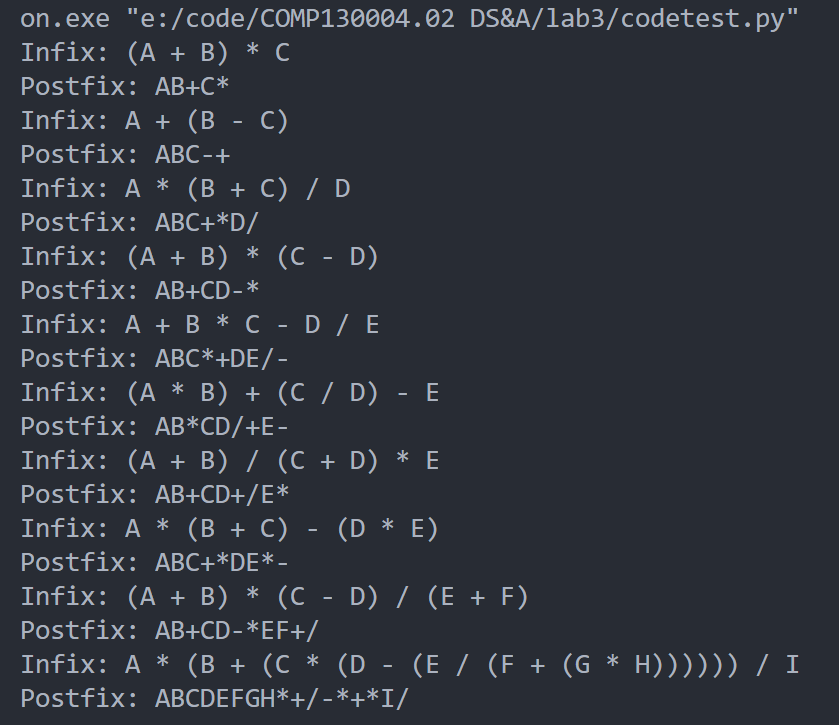
\includegraphics[width=0.8\textwidth]{code1result.png}
    \caption{Test of code 01}
\end{figure}
Run the lower half of the code, we can get the following results:
\begin{figure}[H]
    \centering
    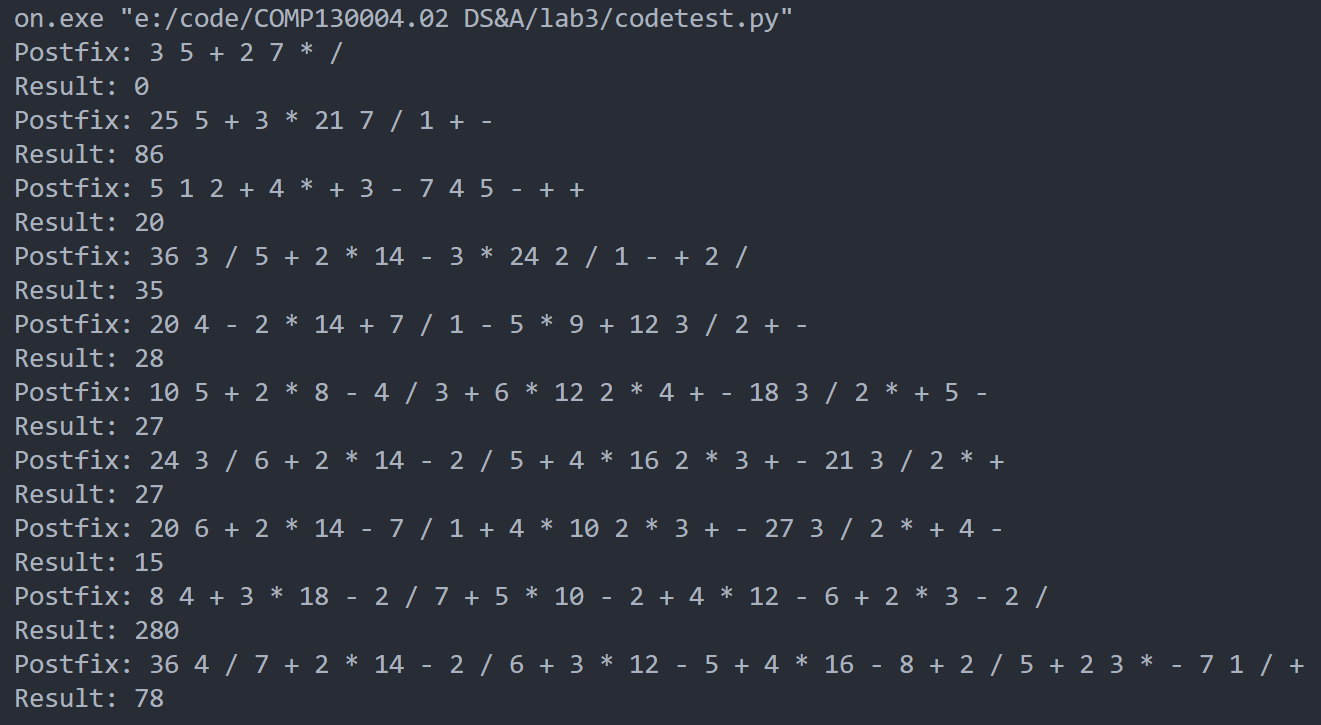
\includegraphics[width=0.8\textwidth]{code2result.png}
    \caption{Test of code 02}
\end{figure}
\textbf{Result analysis:} \\
All the results are correct.\\
For code01, firstly I chose to return a string instead of a list. 
But I found that it is hard to deal with the situation that the input expression is actually numbers instead of alphabets, because numbers with more than one digit cannot be distinguished from one-digit numbers in the string.
So I changed the return type to list and printed the result by joining the list.\\
For code02, I didn't consider the situation that the input expression can be invalid. After I added the try-except statement, the code can deal with invalid expression.
For example, if we input `1 2 + +', the code will print `Error: invalid expression' and return None.\\
By combining the two codes, we can evaluate infix expression easily. The operators supported include small brackets, square brackets, curly brackets 
and $+, -, \times, /, \% \text{(mod)},\wedge \text{(power)} $.
And we can further extend the code to support more operators like `sin', `!', `log' and so on to evaluate more complex expression.\\
\textbf{Conclusion}:\\
By using stack, we can easily convert infix expression to postfix expression and evaluate postfix expression. For conversion, we can use a stack to store operators and pop them according to the priority of operators.
For evaluation, we can use a stack to store operands and pop two operands when meeting an operator. Combined with the two codes, we can evaluate infix expression easily.\\
\end{document}